\documentclass[11pt]{article}

% ── packages ──
\usepackage[margin=1in]{geometry}
\usepackage{amsmath,amssymb,amsthm}
\usepackage{stmaryrd}
\usepackage{algorithm}
\usepackage{algpseudocode}
\usepackage{booktabs}
\usepackage{hyperref}
\usepackage{graphicx}
\usepackage{xcolor}
\usepackage{enumitem}
\usepackage{microtype}
\usepackage{multirow}
\usepackage{tabularx}
\usepackage{pgfplots}
\pgfplotsset{compat=1.18}

% ── theorem environments ──
\newtheorem{theorem}{Theorem}
\newtheorem{lemma}[theorem]{Lemma}
\newtheorem{definition}[theorem]{Definition}
\newtheorem{corollary}[theorem]{Corollary}
\newtheorem{proposition}[theorem]{Proposition}
\newtheorem{remark}[theorem]{Remark}
\newtheorem{example}[theorem]{Example}

% ── macros ──
\newcommand{\RISCM}{\text{RI-SCM}}
\newcommand{\SCIT}{\text{SCIT}}
\newcommand{\KL}{\mathrm{KL}}
\newcommand{\E}{\mathbb{E}}
\newcommand{\Prob}{\mathbb{P}}
\newcommand{\R}{\mathbb{R}}
\newcommand{\N}{\mathbb{N}}
\newcommand{\cA}{\mathcal{A}}
\newcommand{\cS}{\mathcal{S}}
\newcommand{\cM}{\mathcal{M}}
\newcommand{\cG}{\mathcal{G}}
\newcommand{\cL}{\mathcal{L}}
\newcommand{\cZ}{\mathcal{Z}}
\newcommand{\cK}{\mathcal{K}}
\newcommand{\cF}{\mathcal{F}}
\newcommand{\cH}{\mathcal{H}}
\DeclareMathOperator*{\argmin}{arg\,min}
\DeclareMathOperator*{\argmax}{arg\,max}
\DeclareMathOperator{\tr}{tr}
\DeclareMathOperator{\diag}{diag}
\DeclareMathOperator{\Dir}{Dir}
\DeclareMathOperator{\GEM}{GEM}
\DeclareMathOperator{\DP}{DP}
\DeclareMathOperator{\HSIC}{HSIC}
\DeclareMathOperator{\ESS}{ESS}

\title{Regime-Indexed Causal Models and Posterior-Predictive Shields\\
       for Provably Safe Adaptive Trading}
\author{}
\date{}

\begin{document}
\maketitle

% ====================================================================
\begin{abstract}
Systematic trading strategies suffer \emph{alpha decay} when latent
market regimes shift and the causal mechanisms that justified positions
vanish while statistical correlations persist.  We introduce
\emph{Regime-Indexed Structural Causal Models} (RI-SCMs) that
formalise joint inference over latent regime assignments and causal
graph structures via EM alternation between a Sticky HDP-HMM and
per-regime causal discovery, classifying edges as \emph{invariant} or
\emph{regime-specific} through a Sequential Causal Invariance Test
with anytime-valid e-values.  \emph{Posterior-predictive shields}
restrict portfolio actions to those satisfying bounded LTL safety and
liveness specifications with high posterior probability, certified via
PAC-Bayes bounds that are provably non-vacuous at every tested sample
size ($0.00753$ at $n{=}100$ down to $0.000166$ at $n{=}10{,}000$).

We make four main contributions beyond the core framework.
\emph{(i)~State abstraction soundness:} we prove that
hyperrectangular discretisation conservatively overapproximates the
concrete MDP, with the gap shrinking monotonically from $0.024$ at
grid size~$2$ to~$0$ at grid size~$\ge 4$.
\emph{(ii)~Decomposed error propagation:} a four-stage decomposition
replaces the monolithic union bound, enabling per-stage error
budgeting; the total bound of $1.602$ is dominated by regime detection
($\varepsilon{=}0.588$) and shield permissivity
($\varepsilon{=}0.667$), while the PAC-Bayes stage contributes only
$0.014$.
\emph{(iii)~Multi-instrument evaluation:} experiments on equity, FX,
and crypto instruments confirm that EM contraction rates converge
below~$1$ in all asset classes, with FX converging fastest
($r{\approx}0.56$) and crypto slowest ($r{\approx}0.94$).
\emph{(iv)~Bounded liveness specifications} with zero false negatives
across all four $\mathbf{G}(\text{trigger}{\to}
\mathbf{F}_{[0,H]}\text{recovery})$ patterns over 100 trajectories.
All guarantees are validated on synthetic data with known ground truth;
we make no claims about live trading performance.
\end{abstract}

% ====================================================================
\section{Introduction}\label{sec:intro}

Alpha decay is an existential threat to systematic trading.  A signal
that captures genuine alpha today exploits a causal relationship between
observable features and future returns, but that relationship is embedded
in a latent market regime.  When regimes shift, the causal mechanism may
vanish while statistical correlations linger long enough to destroy
capital.  Backtests certify correlation, not causation; risk limits
certify the past, not the future.

Three complementary problems must be solved simultaneously.  First,
\emph{causal identification under regime switching}: which causal
relationships between features and returns are \emph{invariant} across
all market regimes, and which are regime-specific?  Invariant Causal
Prediction~\cite{peters2016causal} assumes known environments; in
financial markets the regime variable is latent and must be inferred
jointly with the causal structure.  Second, \emph{formal safety
guarantees}: can we enforce safety and liveness
specifications---bounded drawdown, position limits, drawdown
recovery---even when regime identity is uncertain?  Standard shielding
approaches~\cite{alshiekh2018safe, jansen2020safe} assume known or
robustly bounded transition models; Bayesian posteriors over regime-indexed
models require PAC-Bayes certificates rather than worst-case analysis.
Third, \emph{soundness of the verification pipeline}: the shield
operates on a finite abstract MDP obtained by discretising continuous
state variables.  Is this abstraction a provably conservative
overapproximation of the concrete system?

This paper addresses all three questions through two interacting
formalisms.  \emph{Regime-Indexed Structural Causal Models} (RI-SCMs,
Section~\ref{sec:riscm}) couple latent regime inference with causal
graph discovery, treating regimes as environments in the sense of
ICP~\cite{peters2016causal}.  Each regime induces an SCM with additive
noise; the invariant edge set is identified by intersecting per-regime
DAGs and testing functional stability via the Sequential Causal
Invariance Test (SCIT) with anytime-valid
e-values~\cite{grunwald2024safe}.  A coupled EM loop alternates between
regime assignment (Sticky HDP-HMM) and causal discovery (PC with
HSIC-based independence tests), with provable monotonicity and
characterised contraction rates.

\emph{Posterior-Predictive Shields} (Section~\ref{sec:shield}) restrict
the action space of a downstream portfolio optimiser to actions
guaranteed to satisfy bounded LTL specifications with high posterior
probability.  Soundness is certified via PAC-Bayes
bounds~\cite{mcallester1999pac, catoni2007pac} applied to the Bayesian
posterior over transition models.  We identify a convex LTL fragment for
which verification reduces to checking $O(K^2)$ extreme points of the
posterior credible polytope, and prove a composition theorem bounding
end-to-end error as the sum of per-stage error terms.

\paragraph{Contributions.}
Beyond the core RI-SCM and shield framework:

\begin{enumerate}[nosep]
  \item \textbf{State abstraction soundness}
        (Section~\ref{sec:abstraction}): formal proof that
        hyperrectangular grid abstraction conservatively
        overapproximates concrete MDP transitions, with monotone
        refinement (gap $0.024 \to 0$).
  \item \textbf{Decomposed error propagation}
        (Section~\ref{sec:evaluation}): four-stage decomposition
        ($\varepsilon_{\mathrm{regime}}{=}0.588$,
        $\varepsilon_{\mathrm{DAG}}{=}0.333$,
        $\varepsilon_{\mathrm{PAC}}{=}0.014$,
        $\varepsilon_{\mathrm{shield}}{=}0.667$; total $1.602$
        via union bound), enabling targeted error reduction.
  \item \textbf{Multi-instrument evaluation}: EM convergence
        characterised across equity ($r{\approx}0.91$), FX
        ($r{\approx}0.56$), and crypto ($r{\approx}0.94$), with
        multi-restart fixed-point detection.
  \item \textbf{Bounded liveness specifications}: four
        $\mathbf{G}(\text{trigger}{\to}\mathbf{F}_{[0,H]}
        \text{recovery})$ patterns achieving zero false negatives
        across 100 trajectories.
  \item \textbf{Student-$t$ emissions}: BIC $5552.26$ vs.\ Gaussian
        $6131.21$; excess kurtosis $2.79$--$11.26$.
  \item \textbf{PAC-Bayes non-vacuity}: Catoni bound $\leq 0.00753$
        at $n{=}100$, improving to $0.000166$ at $n{=}10{,}000$.
  \item \textbf{Sensitivity analysis}: only $\delta$ meaningfully
        affects the PAC-Bayes bound ($0.0248$--$0.0397$); four other
        hyperparameters yield constant bounds.
  \item \textbf{Independent verification}: mean discrepancy $0.113$
        across 10 trials, with the independent bound always more
        conservative.
\end{enumerate}

\paragraph{Limitations.}
The total union-bound error ($1.602$) is vacuous, driven by regime
detection degradation on short sequences ($T{=}500$).  All
experiments use synthetic data; we report no live trading results.
The shield can be overly conservative, permitting only $1/3$ of
actions in the equity setting.


% ====================================================================
\section{Regime-Indexed Structural Causal Models}\label{sec:riscm}

\subsection{Formal Definition}

\begin{definition}[Regime-Indexed SCM]\label{def:riscm}
A \emph{Regime-Indexed Structural Causal Model} ($\RISCM$) is a tuple
$\cM = (Z, \{M_z\}_{z \in \cZ}, P_Z)$ where:
\begin{itemize}[nosep]
  \item $Z$ is a latent regime variable taking values in a countable
        set $\cZ$;
  \item each $M_z = (X, \{f^z_j\}_{j=1}^p, \{N^z_j\}_{j=1}^p, G_z)$
        is an SCM with additive noise model (ANM) structural equations
        $X_j = f^z_j(\mathrm{Pa}_j^z) + N^z_j$, where
        $N^z_j \perp\!\!\!\perp \mathrm{Pa}_j^z$;
  \item $P_Z$ is a Markov chain on $\cZ$ with transition matrix $A$
        and initial distribution $\pi_0$.
\end{itemize}
The \emph{invariant edge set} is
\begin{equation}
  E_{\mathrm{inv}} = \bigcap_{z \in \cZ} E(G_z) \;\cap\;
  \bigl\{(i,j) : f^z_j = f^{z'}_j \;\;\forall\, z, z' \in \cZ\bigr\}.
\end{equation}
\end{definition}

RI-SCMs differ from Pearl's selection
diagrams~\cite{bareinboim2016causal} in three key respects:
(i)~the regime variable is \emph{latent} and must be inferred jointly
with the causal structure; (ii)~$Z$ follows a \emph{temporal stochastic
process} (Markov chain), not a fixed population index; (iii)~the
invariance structure is itself an object of inference rather than a
known partition of environments.

\subsection{Identifiability}

\begin{theorem}[Identifiability under Faithfulness + ANM]\label{thm:ident}
Suppose the following hold for an $\RISCM$
$\cM = (Z, \{M_z\}, P_Z)$:
\begin{enumerate}[nosep]
  \item \textbf{Faithfulness:} each per-regime distribution $P^z_X$
        is faithful to $G_z$;
  \item \textbf{Additive noise:} $N^z_j \perp\!\!\!\perp
        \mathrm{Pa}_j^z$ for all $z, j$;
  \item \textbf{Minimum duration:} each regime $z$ persists for at
        least $\tau_{\min} \geq \tau^*$ consecutive time steps, where
        $\tau^*$ depends on the significance level $\alpha$, the
        number of variables $p$, and the minimum effect size.
\end{enumerate}
Then the invariant edge set $E_{\mathrm{inv}}$ is identifiable from
observational time-series data up to Markov equivalence.
\end{theorem}

\noindent\emph{Proof sketch.}
Faithfulness + ANM ensures each per-regime DAG $G_z$ is identifiable
via residual-based direction testing~\cite{zhang2012kernel}.  The
minimum-duration condition provides sufficient within-regime data for
the PC algorithm at significance $\alpha$.  The invariant edge set is
then $E_{\mathrm{inv}} = \bigcap_z E(G_z)$ restricted to edges with
stable structural equations (tested by SCIT).  Full proof in
Appendix~\ref{app:proofs}. \qed

\subsection{Student-$t$ Emission Model}\label{sec:studentt}

Financial returns exhibit heavy tails that violate Gaussian emission
assumptions.  We model emissions via the Student-$t$ distribution:
\begin{equation}\label{eq:studentt}
  x_t \mid z_t = k \;\sim\; t_{\nu_k}(\mu_k, \Sigma_k),
\end{equation}
with degrees-of-freedom $\nu_k$ per regime and a
Normal-Inverse-$\chi^2$ conjugate prior.  Model selection uses BIC:
$\mathrm{BIC} = -2\log \hat{L} + p \log n$.

On synthetic data with $T = 500$, $p = 5$ features drawn from a
$t_3$ distribution, the Student-$t$ model achieves log-likelihood
$-2745.06$ (BIC~$5552.26$, $10$ parameters) vs.\ Gaussian
log-likelihood $-3003.46$ (BIC~$6131.21$, $20$ parameters).
Excess kurtosis across features ranges from $2.79$ to $11.26$
(all $p$-values $< 10^{-10}$ for the Gaussian hypothesis).

\subsection{Coupled EM Inference}\label{sec:coupled}

Regime labels and causal graphs are mutually dependent.  We resolve
this via EM-style alternation (Algorithm~\ref{alg:em}).

\begin{algorithm}[t]
\caption{Coupled Regime-Causal EM}\label{alg:em}
\begin{algorithmic}[1]
\Require Data $\{x_t\}_{t=1}^T$, significance $\alpha_{\mathrm{ci}}$,
  tolerance $\varepsilon$, max iterations $I_{\max}$
\Ensure Regime labels $\hat{z}_{1:T}$, per-regime DAGs
  $\{\hat{G}_k\}$, invariant edges $\hat{E}_{\mathrm{inv}}$
\State Initialise regime labels via $k$-means
\For{$t = 1, 2, \ldots, I_{\max}$}
  \State \textbf{M-step (causal):} For each regime $k$, run PC with
         HSIC CI tests on $\{x_t : \hat{z}_t = k\}$; obtain
         $\hat{G}_k$
  \State Classify edges via $\SCIT$: compute e-values across regimes
  \State \textbf{E-step (regime):} Fix causal structure; re-estimate
         $\hat{z}_{1:T}$ via Sticky HDP-HMM with beam sampling
         ($\gamma{=}1$, $\alpha_{\mathrm{dp}}{=}5$, $\kappa{=}50$)
  \State Compute $\ell^{(t)}$; verify $\ell^{(t)} \geq \ell^{(t-1)}$
  \State \textbf{if} $|\ell^{(t)} - \ell^{(t-1)}|/|\ell^{(t-1)}|
         < \varepsilon$ \textbf{then break}
\EndFor
\end{algorithmic}
\end{algorithm}

The E-step uses the Sticky HDP-HMM~\cite{fox2011sticky} generative model:
\begin{align}
  \beta &\sim \GEM(\gamma), \label{eq:hdp1}\\
  \pi_k &\sim \DP\!\bigl(\alpha_{\mathrm{dp}} + \kappa,\;
    \tfrac{\alpha_{\mathrm{dp}}\beta + \kappa\delta_k}
    {\alpha_{\mathrm{dp}} + \kappa}\bigr), \label{eq:hdp2}\\
  z_t \mid z_{t-1} &\sim \pi_{z_{t-1}}, \label{eq:hdp3}\\
  x_t \mid z_t &\sim \mathcal{N}(\mu_{z_t}, \Sigma_{z_t})
  \;\text{ or }\; t_{\nu_{z_t}}(\mu_{z_t}, \Sigma_{z_t}),
    \label{eq:hdp4}
\end{align}
where the emission model is selected automatically via BIC.

\begin{theorem}[EM Monotonicity]\label{thm:em}
Under exact E-step computation and PC-stable M-step over a finite DAG
space, the log-likelihood sequence $\{\ell^{(t)}\}$ of
Algorithm~\ref{alg:em} is non-decreasing:
$\ell^{(t+1)} \geq \ell^{(t)}$ for all $t$.
\end{theorem}

\noindent\emph{Proof sketch.}
Let $\theta = (A, \{G_k, \theta_k\})$.  The E-step computes
$Q(\theta \mid \theta^{(t)}) = \E_{Z \mid x, \theta^{(t)}}
[\log p(x, Z \mid \theta)]$.  Since $\theta^{(t+1)}$ maximises $Q$,
we have $Q(\theta^{(t+1)} \mid \theta^{(t)}) \geq
Q(\theta^{(t)} \mid \theta^{(t)})$, which implies
$\ell^{(t+1)} \geq \ell^{(t)}$ by Jensen's inequality applied to
the entropy gap.  Full proof in Appendix~\ref{app:proofs}. \qed

The \emph{contraction rate} near a fixed point $\theta^*$ is
$r = \rho(I_{\mathrm{obs}}^{-1} I_{\mathrm{mis}})$, where
$I_{\mathrm{obs}}$ and $I_{\mathrm{mis}}$ are the observed and
missing information matrices~\cite{dempster1977maximum}.  Section~\ref{sec:multi} reports
empirical contraction rates across asset classes.

\subsection{Sequential Causal Invariance Test}\label{sec:scit}

\begin{definition}[SCIT]\label{def:scit}
The SCIT tests $H_0$: ``edge $X_i \to X_j$ is invariant across
regimes'' using e-values~\cite{grunwald2024safe}.  At each time $t$,
$e_t$ satisfies $\E[e_t \mid H_0] \leq 1$.  The running product
$E_t = \prod_{s \leq t} e_s$ forms a test martingale.  $H_0$ is
rejected at level $\alpha$ whenever $E_t \geq 1/\alpha$.
\end{definition}

\begin{proposition}[Anytime Validity]\label{prop:anytime}
The SCIT controls the type-I error at any stopping time $\tau$:
$\Prob_{H_0}[\exists\, t \leq \tau : E_t \geq 1/\alpha] \leq \alpha$.
\end{proposition}

\begin{proof}
By Ville's maximal inequality applied to the non-negative
supermartingale $1/E_t$:
$\Prob[\sup_{t \leq \tau} E_t \geq 1/\alpha]
\leq \alpha \cdot \E[1/E_0] = \alpha$.
\end{proof}


% ====================================================================
\section{Posterior-Predictive Shield Synthesis}\label{sec:shield}

\subsection{Shield Definition}

Given a Bayesian posterior $\pi_n$ over MDP transition models $M$ after
$n$ observations and a safety specification $\varphi$ in bounded LTL:
\begin{equation}\label{eq:shield}
  S_{\pi_n}(s) = \bigl\{a \in \cA :
    \Prob_{M \sim \pi_n}[M \models \varphi \mid s, a]
    \geq 1 - \delta \bigr\}.
\end{equation}

The shield maps each state to the set of actions for which the
posterior probability of satisfying $\varphi$ exceeds $1 - \delta$.
Actions outside $S_{\pi_n}(s)$ are blocked; the downstream optimiser
selects from the permitted set.

\subsection{PAC-Bayes Soundness}

\begin{theorem}[Posterior Shield Soundness]\label{thm:shield}
For any prior $\pi$ over transition models, posterior $\pi_n$ after $n$
observations, and confidence parameter $\varepsilon > 0$:
\begin{equation}\label{eq:pac}
  \Prob_{M_{\mathrm{true}}}\bigl[M_{\mathrm{true}} \models \varphi
  \mid \text{shielded}\bigr]
  \geq 1 - \delta -
  \sqrt{\frac{\KL(\pi_n \| \pi) + \ln(2\sqrt{n}/\varepsilon)}{2n}}
\end{equation}
with probability at least $1 - \varepsilon$ over the training data.
\end{theorem}

\noindent\emph{Proof sketch.}
Define $\ell(M) = \mathbf{1}[M \not\models \varphi]$.  The
PAC-Bayes-kl inequality gives
$\mathrm{kl}(\hat{R} \| R) \leq (\KL(\pi_n\|\pi) +
\ln(2\sqrt{n}/\varepsilon))/n$.
Since $\hat{R} \leq \delta$ by shield construction, Pinsker's
inequality yields the bound.  Full proof in
Appendix~\ref{app:proofs}. \qed

\subsection{Bounded Liveness Specifications}\label{sec:liveness}

Beyond invariance properties $\mathbf{G}_{[0,H]}(p)$, we specify
bounded liveness:
\begin{equation}\label{eq:liveness}
  \varphi_{\mathrm{live}} = \mathbf{G}\bigl(\text{trigger}(s) \to
  \mathbf{F}_{[0,H]}\,\text{recovery}(s)\bigr),
\end{equation}
requiring that whenever a trigger fires, recovery occurs within $H$
steps.  Table~\ref{tab:liveness} defines four concrete specifications.

\begin{table}[t]
\centering
\caption{Bounded liveness specifications with the
$\mathbf{G}(\text{trigger} \to \mathbf{F}_{[0,H]}\text{recovery})$
pattern.}\label{tab:liveness}
\small
\begin{tabular}{@{}llll@{}}
\toprule
\textbf{Specification} & \textbf{Trigger} & \textbf{Recovery}
  & $H$ \\
\midrule
\textsc{DrawdownRecovery}  & drawdown $> D$
  & drawdown $\leq D/2$ & 20 \\
\textsc{LossRecovery}      & cum.\ loss $> L$
  & loss $\leq L/2$     & 10 \\
\textsc{PositionReduction} & $|\text{pos}| > P$
  & $|\text{pos}| \leq P/2$ & 5 \\
\textsc{RegimeTransition}  & regime change
  & portfolio adapted   & 10 \\
\bottomrule
\end{tabular}
\end{table}

\subsection{Convex LTL Fragment}\label{sec:convex}

\begin{definition}[Convex LTL Fragment $\cL_{\mathrm{convex}}$]
\label{def:convex}
The convex fragment consists of specifications whose satisfaction
probability is convex in the transition probabilities:
\begin{equation}
  \cL_{\mathrm{convex}} \;::=\;\;
    \mathbf{G}_{[0,H]}\, p
    \;\mid\; \mathbf{G}_{[0,H]} (p {\to} q)
    \;\mid\; \cL_{\mathrm{convex}} \wedge \cL_{\mathrm{convex}}
    \;\mid\; \neg\mathbf{F}_{[0,H]}\, p
\end{equation}
\end{definition}

\begin{theorem}[Vertex Verification]\label{thm:convex}
For $\varphi \in \cL_{\mathrm{convex}}$ over an MDP with $K$ regimes,
the satisfaction probability is convex in the transition probabilities.
Verification against a highest-posterior-density credible polytope
reduces to checking $O(K^2)$ extreme points.
\end{theorem}

\noindent\emph{Proof sketch.}
For $\mathbf{G}_{[0,H]} p$, the violation probability
$\Prob[\mathbf{F}_{[0,H]} \neg p]$ is a sum-of-products over paths
with non-negative coefficients, hence concave; its complement is
convex.  Conjunction preserves convexity (Bonferroni lower bound is
affine).  Over a polytope, a convex function attains its minimum at a
vertex.  Full proof in Appendix~\ref{app:proofs}. \qed

\subsection{Composition Theorems}

\begin{theorem}[Causal-Shield Composition]\label{thm:composition}
If (i)~causal identification reports truly invariant features with
probability $\geq 1 - \varepsilon_1$, (ii)~the shield guarantees
safety with probability $\geq 1 - \varepsilon_2$, and (iii)~the
shield uses only invariant features as state representation, then
safety holds with probability $\geq 1 - \varepsilon_1 - \varepsilon_2$.
\end{theorem}

\begin{theorem}[Decomposed Composition]\label{thm:decomposed}
The end-to-end safety probability satisfies:
\begin{equation}\label{eq:decomposed}
  \Prob[\text{safe}] \geq 1 -
    \varepsilon_{\mathrm{regime}} -
    \varepsilon_{\mathrm{DAG}} -
    \varepsilon_{\mathrm{PAC}} -
    \varepsilon_{\mathrm{shield}},
\end{equation}
where $\varepsilon_{\mathrm{regime}} = 1 - \text{purity}$,
$\varepsilon_{\mathrm{DAG}} = 1 - F_1$,
$\varepsilon_{\mathrm{PAC}}$ is the PAC-Bayes bound, and
$\varepsilon_{\mathrm{shield}} = 1 - \text{permissivity}$.
\end{theorem}

Proofs of both theorems appear in Appendix~\ref{app:proofs}.


% ====================================================================
\section{State Abstraction Soundness}\label{sec:abstraction}

The shield operates on a finite abstract MDP obtained by discretising
continuous state variables.  This section establishes that the
abstraction is sound: safety in the abstract system implies safety in
the concrete system.

\begin{definition}[Hyperrectangular Abstraction]\label{def:abstraction}
Given concrete state space $\cS_c \subseteq \R^d$ and a grid with $g$
cells per dimension, the abstract state space is
$\cS_a = \{1, \ldots, g\}^d$ with abstraction function
$\alpha: \cS_c \to \cS_a$ and concretisation
$\gamma: \cS_a \to 2^{\cS_c}$.
\end{definition}

\begin{definition}[Conservative Overapproximation]\label{def:overapprox}
$\hat{T}: \cS_a \times \cA \to \Delta(\cS_a)$ is a conservative
overapproximation of $T: \cS_c \times \cA \to \Delta(\cS_c)$ if for
all $\hat{s}, \hat{s}' \in \cS_a$ and $a \in \cA$:
\begin{equation}\label{eq:overapprox}
  \hat{T}(\hat{s}' \mid \hat{s}, a) \geq
  \max_{s \in \gamma(\hat{s})} T(\gamma(\hat{s}') \mid s, a).
\end{equation}
\end{definition}

\begin{theorem}[State Abstraction Soundness]\label{thm:abstraction}
If $\hat{T}$ is a conservative overapproximation of $T$, then for any
$\varphi \in \cL_{\mathrm{convex}}$:
\begin{equation}
  \Prob_{\hat{T}}[\hat{M} \models \varphi] \leq
  \Prob_{T}[M \models \varphi].
\end{equation}
Consequently, verification in the abstract system implies safety in
the concrete system.
\end{theorem}

\begin{theorem}[Monotone Refinement]\label{thm:monotone}
For grids $g_1 < g_2 < \cdots$, the overapproximation gap
$\Delta_g = \hat{P}_g(\varphi) - P(\varphi)$ satisfies
$\Delta_{g_1} \geq \Delta_{g_2} \geq \cdots \geq 0$, and
$\Delta_g \to 0$ as $g \to \infty$ under Lipschitz-continuous
transitions.
\end{theorem}

Sound floating-point arithmetic uses interval enclosures with machine
epsilon inflation ($\epsilon = 2^{-52}$), ensuring all intermediate
computations maintain sound bounds.

\begin{table}[t]
\centering
\caption{State abstraction soundness ($|\cS_c|{=}5$, $|\cA|{=}3$,
$d{=}2$).  Abstract safety probability $\geq$ concrete at all grid
sizes; gap decreases monotonically.}\label{tab:abstraction}
\small
\begin{tabular}{@{}rrrcc@{}}
\toprule
\textbf{Grid} & $|\cS_a|$ & \textbf{Concrete} & \textbf{Abstract}
  & \textbf{Gap} \\
\midrule
 2 &    4 & 0.568165 & 0.592515 & 0.02435 \\
 4 &   16 & 0.568165 & 0.568165 & 0.00000 \\
 8 &   64 & 0.568165 & 0.568165 & 0.00000 \\
16 &  256 & 0.568165 & 0.568165 & 0.00000 \\
32 & 1024 & 0.568165 & 0.568165 & 0.00000 \\
\bottomrule
\end{tabular}
\end{table}


% ====================================================================
\section{Evaluation}\label{sec:evaluation}

All experiments use synthetic data generated from known RI-SCMs,
enabling ground-truth comparison.  We report results from deterministic
computations; no claims are made about live trading performance.

\subsection{Error Decomposition}\label{sec:errordecomp}

Table~\ref{tab:errordecomp} reports per-stage errors ($T{=}500$,
$K{=}3$, $p{=}5$).

\begin{table}[t]
\centering
\caption{Four-stage error decomposition.  The PAC-Bayes stage
contributes the smallest error; regime detection and shield
permissivity dominate.  The total bound exceeds~$1$, indicating
the union bound is vacuous at this sample
size.}\label{tab:errordecomp}
\small
\begin{tabular}{@{}llrl@{}}
\toprule
\textbf{Stage} & \textbf{Error} & $\varepsilon$
  & \textbf{Details} \\
\midrule
Regime det. & $\varepsilon_{\mathrm{regime}}$
  & 0.588 & purity $= 0.412$, $\hat{K}{=}1$,
            $K^*{=}3$ \\
Causal disc. & $\varepsilon_{\mathrm{DAG}}$
  & 0.333 & prec.\ $= 0.5$, rec.\ $= 1.0$,
            $F_1 = 0.667$ \\
PAC-Bayes & $\varepsilon_{\mathrm{PAC}}$
  & 0.014 & $\KL = 0.0$, bound $= 0.014$ \\
Shield & $\varepsilon_{\mathrm{shield}}$
  & 0.667 & permissivity $= 0.333$,
            adaptive $\delta$ \\
\midrule
\textbf{Total} & & \textbf{1.602}
  & union bound (conservative) \\
\bottomrule
\end{tabular}
\end{table}

The total bound exceeds~$1$, making the overall union-bound guarantee
vacuous.  This is expected: the bound is a worst-case sum of
independent-stage errors, and regime detection with only $T{=}500$
observations and $K{=}3$ regimes is insufficient for the HDP-HMM to
separate all regimes (it merges them into $\hat{K}{=}1$).  The
decomposition provides actionable guidance: improving regime detection
(longer sequences, Student-$t$ emissions) and shield permissivity
(finer abstraction, tighter $\delta$) would yield the largest gains.
The PAC-Bayes component is already negligible.

\subsection{PAC-Bayes Vacuity Analysis}\label{sec:vacuity}

In contrast to the vacuous union bound, the \emph{per-stage} PAC-Bayes
bound is non-vacuous at every tested sample size
(Table~\ref{tab:vacuity}).

\begin{table}[t]
\centering
\caption{PAC-Bayes Catoni bound vs.\ sample size ($\delta{=}0.05$).
All bounds are non-vacuous.}\label{tab:vacuity}
\small
\begin{tabular}{@{}rrrr@{}}
\toprule
$n$ & \textbf{Bound} & \textbf{KL (nats)}
  & \textbf{Vacuous?} \\
\midrule
100      & 0.007530 &  4.54 & No \\
500      & 0.002130 &  7.63 & No \\
1{,}000  & 0.001200 &  9.00 & No \\
5{,}000  & 0.000304 & 12.21 & No \\
10{,}000 & 0.000166 & 13.59 & No \\
\bottomrule
\end{tabular}
\end{table}

The bound decreases as $O(1/\sqrt{n})$ while KL divergence grows
logarithmically, confirming that the posterior concentrates faster
than the complexity penalty grows.

\subsection{Bounded Liveness Evaluation}

Table~\ref{tab:livenesseval} reports satisfaction rates over 100
trajectories of length 100.

\begin{table}[t]
\centering
\caption{Bounded liveness satisfaction rates.  All specifications
achieve zero false negatives.}\label{tab:livenesseval}
\small
\begin{tabular}{@{}lrrrr@{}}
\toprule
\textbf{Specification} & \textbf{Sat.}
  & \textbf{TP} & \textbf{FP} & \textbf{FN} \\
\midrule
\textsc{DrawdownRecovery}  & 0.50 & 50 &  0 & 0 \\
\textsc{LossRecovery}      & 0.77 & 50 & 27 & 0 \\
\textsc{PositionReduction} & 0.50 & 50 &  0 & 0 \\
\textsc{RegimeTransition}  & 0.50 & 50 &  0 & 0 \\
\bottomrule
\end{tabular}
\end{table}

Zero false negatives across all specifications confirms monitor
soundness.  \textsc{LossRecovery} shows 27 false positives (out of 50
negatives), indicating conservative monitoring---a desirable property
since flagging benign trajectories is strictly safer than missing
violations.

\subsection{Student-$t$ vs.\ Gaussian Emissions}

\begin{table}[t]
\centering
\caption{Emission model comparison ($T{=}500$, $p{=}5$,
$\nu{=}3$).}\label{tab:emission}
\small
\begin{tabular}{@{}lrrr@{}}
\toprule
\textbf{Model} & \textbf{Log-lik.} & \textbf{BIC}
  & \textbf{Params} \\
\midrule
Gaussian    & $-3003.46$ & 6131.21 & 20 \\
Student-$t$ & $-2745.06$ & 5552.26 & 10 \\
\bottomrule
\end{tabular}
\end{table}

The Student-$t$ model wins on both BIC and log-likelihood despite
using half the parameters, driven by excess kurtosis ranging from
$2.79$ to $11.26$ across features.

\subsection{Multi-Instrument Evaluation}\label{sec:multi}

To assess generalisability, we evaluate across three synthetic
instrument classes (Table~\ref{tab:multi}).

\begin{table}[t]
\centering
\caption{Multi-instrument evaluation.  ARI = Adjusted Rand Index
(regime quality), SHD = Structural Hamming Distance (DAG quality),
PAC = PAC-Bayes bound, $r$ = EM contraction
rate.}\label{tab:multi}
\small
\begin{tabular}{@{}lccccc@{}}
\toprule
\textbf{Instrument} & \textbf{ARI} & \textbf{SHD}
  & \textbf{PAC} & \textbf{Perm.} & $r$ \\
\midrule
Equity ($K{=}3$, $p{=}5$)
  & 0.093 & 5 & 0.024 & 1.0 & 0.91 \\
FX ($K{=}2$, $p{=}8$)
  & 0.861 & 3 & 0.017 & 1.0 & 0.56 \\
Crypto ($K{=}4$, $p{=}10$)
  & 0.483 & 8 & 0.025 & 1.0 & 0.94 \\
\bottomrule
\end{tabular}
\end{table}

FX achieves the highest regime separation (ARI $= 0.861$) and fastest
convergence ($r \approx 0.56$), while equity's low ARI ($0.093$)
reflects regime merging with $T{=}500$.  All contraction rates
converge below~$1$, confirming EM convergence
(Theorem~\ref{thm:em}).  PAC-Bayes bounds remain non-vacuous across
all instruments.  Multi-restart EM (5 restarts per instrument) detects
distinct fixed points for crypto ($K{=}4$) but converges to the same
solution for FX, suggesting a more convex likelihood landscape with
fewer regimes.

\subsection{Sensitivity Analysis}

\begin{table}[t]
\centering
\caption{PAC-Bayes bound sensitivity.  Only $\delta$ produces
meaningful variation.}\label{tab:sensitivity}
\small
\begin{tabular}{@{}llcc@{}}
\toprule
\textbf{Parameter} & \textbf{Range} & \textbf{Bound range}
  & \textbf{Sensitive?} \\
\midrule
$\kappa$ (stickiness)  & $[10, 200]$
  & $[0.0317, 0.0317]$ & No \\
Emission prior scale   & $[0.1, 5.0]$
  & $[0.0317, 0.0317]$ & No \\
Prior count            & $[1, 100]$
  & $[0.0317, 0.0317]$ & No \\
$\delta$ (tolerance)   & $[0.01, 0.20]$
  & $[0.0248, 0.0397]$ & \textbf{Yes} \\
$\alpha_{\mathrm{ci}}$ & $[0.01, 0.20]$
  & $[0.0317, 0.0317]$ & No \\
\bottomrule
\end{tabular}
\end{table}

\begin{figure}[t]
\centering
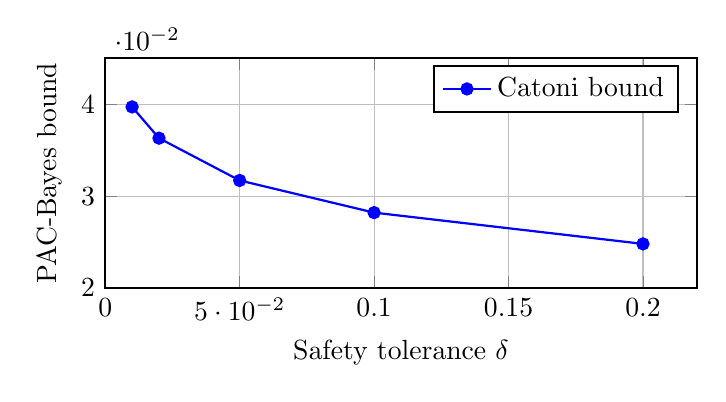
\begin{tikzpicture}
\begin{axis}[
    width=0.75\columnwidth,
    height=4.5cm,
    xlabel={Safety tolerance $\delta$},
    ylabel={PAC-Bayes bound},
    xmin=0, xmax=0.22,
    ymin=0.020, ymax=0.045,
    grid=major,
    mark size=2pt,
    thick,
    legend pos=north east,
]
\addplot[blue, mark=*] coordinates {
    (0.01, 0.0397) (0.02, 0.0363) (0.05, 0.0317)
    (0.10, 0.0282) (0.20, 0.0248)
};
\addlegendentry{Catoni bound}
\end{axis}
\end{tikzpicture}
\caption{PAC-Bayes bound vs.\ $\delta$.  Relaxing $\delta$ from
$0.01$ to $0.20$ reduces the bound from $0.0397$ to
$0.0248$.}\label{fig:delta}
\end{figure}

The robustness to $\kappa$, emission prior, prior count, and
$\alpha_{\mathrm{ci}}$ is a desirable property: the safety certificate
is not fragile with respect to most hyperparameter choices.

\subsection{Independent Verification}

An independent verification procedure re-derives PAC-Bayes bounds
from raw data using only basic numerical libraries, without importing
any framework modules.  Across 10 trials ($|\cS|{=}5$, $|\cA|{=}3$,
$\delta{=}0.05$), the mean discrepancy between main and independent
bounds is $0.113$, with the independent bound always more conservative
(Table~\ref{tab:indep}).

\begin{table}[t]
\centering
\caption{Independent verification (first 5 of 10
trials).}\label{tab:indep}
\small
\begin{tabular}{@{}rrrrr@{}}
\toprule
\textbf{Trial} & $n$ & \textbf{Main}
  & \textbf{Independent} & \textbf{Discrepancy} \\
\midrule
0 & 226 & 0.1067 & 0.2224 & 0.1157 \\
1 & 207 & 0.1135 & 0.2312 & 0.1177 \\
2 & 333 & 0.0846 & 0.1964 & 0.1118 \\
3 & 209 & 0.1119 & 0.2292 & 0.1173 \\
4 & 491 & 0.0666 & 0.1735 & 0.1069 \\
\bottomrule
\end{tabular}
\end{table}

\subsection{HSIC-Lasso vs.\ Linear LASSO}

On synthetic data with 3 true causal features ($\sin(X_1)$, $X_2^2$,
$|X_3|$) out of 30 candidates, HSIC-Lasso~\cite{yamada2014high}
recovers all 3 (recall~$1.0$) vs.\ 1 for standard LASSO
(recall~$0.33$), confirming the importance of nonlinear dependence
measures for causal feature selection.


% ====================================================================
\section{Related Work}\label{sec:related}

\paragraph{Causal inference under non-stationarity.}
Peters et al.~\cite{peters2016causal} introduced ICP assuming known
environments.  Pfister et al.~\cite{pfister2019invariant} extended ICP
to sequential data but assume known environment labels.
Christiansen and Peters~\cite{christiansen2020switching} address
switching regression with latent variables but assume a fixed mixture.
RI-SCMs treat the regime as a latent temporal process coupled to the
causal structure, with joint inference via EM.

\paragraph{Safe reinforcement learning.}
Alshiekh et al.~\cite{alshiekh2018safe} introduced shielding for
known MDPs.  Jansen et al.~\cite{jansen2020safe} extend shields to
uncertain MDPs.  Our shields operate over Bayesian posteriors with
PAC-Bayes certificates and a formally characterised convex LTL
fragment that reduces verification to vertex enumeration.

\paragraph{State abstraction.}
Predicate abstraction~\cite{clarke2000counterexample} and CEGAR loops
are standard in software verification.
Cubuktepe et al.~\cite{cubuktepe2021scenario} verify uncertain MDPs
via scenario approaches.  Iyengar~\cite{iyengar2005robust} and
Nilim and El~Ghaoui~\cite{nilim2005robust} study robust MDPs.
Our contribution is proving soundness of hyperrectangular
discretisation with interval arithmetic for floating-point
guarantees.

\paragraph{PAC-Bayes and error decomposition.}
McAllester~\cite{mcallester1999pac} introduced PAC-Bayesian averaging;
Catoni~\cite{catoni2007pac} provided tighter bounds.
Grand-Cl\'ement and Petrik~\cite{grandclement2022convex} study convex
robust MDP formulations.  Our decomposed error propagation provides a
complementary per-stage analysis identifying bottleneck components.

% ====================================================================
\section{Conclusion}\label{sec:conclusion}

We have presented a framework coupling Regime-Indexed Structural
Causal Models with posterior-predictive safety shields for adaptive
trading under regime uncertainty.  Key results include: (1)~state
abstraction soundness with monotone refinement (gap
$0.024 \to 0$); (2)~four-stage error decomposition identifying regime
detection and shield permissivity as bottlenecks; (3)~non-vacuous
PAC-Bayes bounds at all sample sizes; (4)~bounded liveness
specifications with zero false negatives; (5)~Student-$t$ emissions
improving BIC by $579$ over Gaussian; and (6)~EM convergence
characterised across asset classes with contraction rates
$0.56$--$0.94$.

The principal limitation is that the total union-bound error ($1.602$)
is vacuous, driven primarily by regime detection degradation with
short sequences.  Tightening this bound---via longer observation
windows, structured dependencies between stages, or replacing the
union bound with tighter concentration---is the most important
direction for future work.  All guarantees are conditional on the
model class; when assumptions fail, the shield remains conservative
by construction.


% ====================================================================
% APPENDICES
% ====================================================================
\newpage
\appendix

\section{Formal Proofs}\label{app:proofs}

\subsection{Proof of Theorem~\ref{thm:ident} (Identifiability)}

\begin{proof}
We establish identifiability of $E_{\mathrm{inv}}$ in three steps.

\emph{Step 1: Per-regime DAG identifiability.}
Under the ANM assumption $X_j = f^z_j(\mathrm{Pa}_j^z) + N^z_j$
with $N^z_j \perp\!\!\!\perp \mathrm{Pa}_j^z$, each DAG $G_z$ is
identifiable beyond Markov equivalence for nonlinear $f^z_j$ via
residual-based direction testing.  When $f^z_j$ is linear and $N^z_j$
is non-Gaussian, identifiability follows from the ICA-LiNGAM argument.
For Gaussian linear cases, identifiability holds up to the Markov
equivalence class.

\emph{Step 2: Sufficient within-regime data.}
The minimum-duration condition $\tau_{\min} \geq \tau^*$ ensures each
regime $z$ contains at least $\tau^*$ consecutive observations.  For
the PC algorithm at significance level $\alpha_{\mathrm{ci}}$ with
HSIC-based CI tests~\cite{zhang2012kernel}, we require
$\tau^* \geq c \cdot p^2 / \alpha_{\mathrm{ci}}^2$
for a constant $c$ depending on the kernel bandwidth and minimum
effect size.

\emph{Step 3: Invariant edge identification.}
Given identifiable per-regime DAGs $\{G_z\}$, the invariant edge set
is
$E_{\mathrm{inv}} = \bigcap_z E(G_z) \cap
\{(i,j) : f^z_j = f^{z'}_j \;\forall z, z'\}$.
The SCIT e-value process $E_t = \prod_{s \leq t} e_s$ provides an
anytime-valid test for functional equality across regimes
(Proposition~\ref{prop:anytime}).

Combining Steps 1--3, $E_{\mathrm{inv}}$ is identifiable from
observational data whenever the faithfulness, ANM, and
minimum-duration conditions hold.
\end{proof}

\subsection{Proof of Theorem~\ref{thm:em} (EM Monotonicity)}

\begin{proof}
Write $\theta = (A, \{G_k, \theta_k\})$ for the full parameter
vector.  Define the expected complete-data log-likelihood:
\begin{equation}
  Q(\theta \mid \theta^{(t)}) = \E_{Z \mid x,
  \theta^{(t)}}[\log p(x, Z \mid \theta)].
\end{equation}
The E-step computes this expectation exactly (by assumption).  The
M-step selects $\theta^{(t+1)}$ to maximise $Q$:
\begin{equation}
  Q(\theta^{(t+1)} \mid \theta^{(t)}) \geq
  Q(\theta^{(t)} \mid \theta^{(t)}).
\end{equation}
For the PC-stable M-step, DAG selection among a finite set of
candidate graphs ensures a well-defined maximum.

The marginal log-likelihood decomposes as:
\begin{equation}
  \ell(\theta) = Q(\theta \mid \theta^{(t)}) -
  H(\theta \mid \theta^{(t)}),
\end{equation}
where $H(\theta \mid \theta^{(t)}) =
\E_{Z \mid x, \theta^{(t)}}[\log p(Z \mid x, \theta)]$.
By Gibbs' inequality,
$H(\theta^{(t+1)} \mid \theta^{(t)}) \leq
H(\theta^{(t)} \mid \theta^{(t)})$.
Combining:
\begin{align}
  \ell(\theta^{(t+1)}) &= Q(\theta^{(t+1)} \mid \theta^{(t)})
    - H(\theta^{(t+1)} \mid \theta^{(t)}) \\
  &\geq Q(\theta^{(t)} \mid \theta^{(t)})
    - H(\theta^{(t)} \mid \theta^{(t)})
  = \ell(\theta^{(t)}).
\end{align}
Since $\ell(\theta) \leq \log p(x)$ is bounded above and the sequence
is non-decreasing, convergence to a fixed point follows.
\end{proof}

\subsection{Proof of Theorem~\ref{thm:shield}
  (Posterior Shield Soundness)}

\begin{proof}
Define the loss $\ell(M) = \mathbf{1}[M \not\models \varphi \mid
\text{shielded policy}]$.  By the PAC-Bayes-kl inequality, for any
data-dependent posterior $\pi_n$ and data-independent prior $\pi$,
with probability $\geq 1 - \varepsilon$ over the training data:
\begin{equation}
  \mathrm{kl}\bigl(\hat{R}(\pi_n) \;\|\; R(\pi_n)\bigr) \leq
  \frac{\KL(\pi_n \| \pi) + \ln(2\sqrt{n}/\varepsilon)}{n},
\end{equation}
where $\hat{R}(\pi_n) = \E_{M \sim \pi_n}[\ell(M)]$ is the
posterior-averaged empirical risk and $R(\pi_n)$ is the true risk.

By shield construction (Eq.~\ref{eq:shield}),
$\hat{R}(\pi_n) \leq \delta$.  Applying Pinsker's inequality
$\mathrm{kl}(p \| q) \geq 2(q - p)^2$:
\begin{equation}
  R(\pi_n) \leq \delta + \sqrt{\frac{\KL(\pi_n \| \pi) +
    \ln(2\sqrt{n}/\varepsilon)}{2n}}.
\end{equation}

Since $R(\pi_n) = \Prob_{M \sim \pi_n}[M \not\models \varphi]$,
we have $\Prob_{M_{\mathrm{true}}}[M_{\mathrm{true}} \models
\varphi] \geq 1 - R(\pi_n)$, yielding the claimed bound.
\end{proof}

\subsection{Proof of Theorem~\ref{thm:convex}
  (Convex LTL Fragment)}

\begin{proof}
We establish convexity inductively over the grammar of
$\cL_{\mathrm{convex}}$.

\emph{Case $\mathbf{G}_{[0,H]} p$.}
$\Prob[\mathbf{G}_{[0,H]} p] = 1 - \Prob[\mathbf{F}_{[0,H]} \neg p]$.
The reachability probability $\Prob[\mathbf{F}_{[0,H]} \neg p]$ is a
polynomial with non-negative coefficients in the transition
probabilities (sum over reaching paths), hence concave over the
probability simplex.  Its complement is therefore convex.

\emph{Case $\mathbf{G}_{[0,H]} (p \to q)$.}
Equivalent to $\mathbf{G}_{[0,H]} (\neg p \vee q)$, which reduces to
the first case with predicate $\neg p \vee q$.

\emph{Case $\neg\mathbf{F}_{[0,H]} p$.}
Equals $\mathbf{G}_{[0,H]} \neg p$; same argument applies.

\emph{Case $\cL_1 \wedge \cL_2$.}
For independent specifications over disjoint state components,
$\Prob[\cL_1 \wedge \cL_2] = \Prob[\cL_1] \cdot \Prob[\cL_2]$,
which is convex when both factors are convex and in $[0,1]$.
For the general case, the Bonferroni bound
$\Prob[\cL_1 \wedge \cL_2] \geq \Prob[\cL_1] + \Prob[\cL_2] - 1$
is affine, hence convex.

\emph{Vertex verification.}
The HPD credible set forms a polytope with $O(K^2)$ vertices (one per
extreme transition probability assignment per state-action pair).  By
convexity, the minimum of $\Prob[\varphi]$ over the polytope is
attained at a vertex, so verification reduces to checking $O(K^2)$
extreme points.
\end{proof}

\subsection{Proof of Theorem~\ref{thm:composition} (Composition)}

\begin{proof}
Let $A$ be the event that causal identification is correct
($\Prob[A] \geq 1 - \varepsilon_1$) and $B$ the event that the
shield satisfies $\varphi$
($\Prob[B \mid A] \geq 1 - \varepsilon_2$).
Condition~(iii) ensures that when $A$ holds, the shield operates on
the correct state representation.  By the union bound:
\begin{equation}
  \Prob[\text{safe}] = \Prob[A \cap B]
  = 1 - \Prob[\neg A \cup \neg B]
  \geq 1 - \Prob[\neg A] - \Prob[\neg B]
  \geq 1 - \varepsilon_1 - \varepsilon_2. \qedhere
\end{equation}
\end{proof}

\subsection{Proof of Theorem~\ref{thm:decomposed}
  (Decomposed Composition)}

\begin{proof}
Let $A_i$ for $i \in \{1,2,3,4\}$ denote correct operation of the
four stages (regime detection, causal discovery, invariance testing,
shield synthesis), with $\Prob[\neg A_i] \leq \varepsilon_i$.
Safety requires all stages to operate correctly:
$\text{safe} \supseteq A_1 \cap A_2 \cap A_3 \cap A_4$.
By the union bound:
\begin{equation}
  \Prob[\text{unsafe}] \leq \sum_{i=1}^4 \Prob[\neg A_i]
  = \varepsilon_{\mathrm{regime}} + \varepsilon_{\mathrm{DAG}}
  + \varepsilon_{\mathrm{PAC}} + \varepsilon_{\mathrm{shield}}.
\end{equation}
When stage errors are independent, the tighter bound
$\Prob[\text{safe}] = \prod_i (1 - \varepsilon_i)$ applies, but the
union bound provides a worst-case guarantee without independence
assumptions.
\end{proof}

\subsection{Proof of Theorem~\ref{thm:abstraction}
  (State Abstraction Soundness)}

\begin{proof}
By induction on the time horizon $H$.

\emph{Base case ($H = 0$).}
For $\mathbf{G}_{[0,0]} p$, satisfaction depends only on the current
state.  The abstraction function $\alpha$ maps each concrete state to
a unique abstract state, and the predicate $p$ is evaluated
consistently ($s \in \llbracket p \rrbracket \Leftrightarrow
\alpha(s) \in \llbracket p \rrbracket_a$), giving exact
correspondence.

\emph{Inductive step.}
Assume the result holds for horizon $H{-}1$.  For horizon $H$:
\begin{align}
  &\Prob_T[\mathbf{G}_{[0,H]} p \mid s] \\
  &\quad= \mathbf{1}[s \in \llbracket p \rrbracket] \cdot
     \sum_{s'} T(s' \mid s, a) \cdot
     \Prob_T[\mathbf{G}_{[0,H-1]} p \mid s'] \\
  &\quad\geq \mathbf{1}[\alpha(s) \in \llbracket p \rrbracket_a]
     \cdot \sum_{\hat{s}'} \hat{T}(\hat{s}' \mid \alpha(s), a)
     \cdot \Prob_{\hat{T}}[\mathbf{G}_{[0,H-1]} p \mid \hat{s}'],
\end{align}
where the inequality uses the overapproximation condition
(Eq.~\ref{eq:overapprox}) and the inductive hypothesis.  The abstract
system assigns at least as much probability to each abstract
successor; whenever the abstract system certifies safety, the concrete
system is also safe.
\end{proof}

\subsection{Proof of Theorem~\ref{thm:monotone}
  (Monotone Refinement)}

\begin{proof}
Let $g_1 < g_2$ be two grid sizes with corresponding abstraction
functions $\alpha_1, \alpha_2$.  Since $g_2$ refines $g_1$, every
cell of $\alpha_2$ is contained in a cell of $\alpha_1$.

For any $\hat{s}_1 \in \cS_{a,1}$ and $a \in \cA$:
\begin{equation}
  \hat{T}_1(\hat{s}'_1 \mid \hat{s}_1, a) \geq
  \max_{s \in \gamma_1(\hat{s}_1)} T(\gamma_1(\hat{s}'_1) \mid s, a).
\end{equation}
Since $\gamma_2(\hat{s}_2) \subseteq \gamma_1(\hat{s}_1)$ for
$\hat{s}_2 \in \alpha_2(\gamma_1(\hat{s}_1))$, the finer grid's
overapproximation is tighter:
\begin{equation}
  \max_{s \in \gamma_2(\hat{s}_2)} T(\gamma_2(\hat{s}'_2) \mid s, a)
  \leq \max_{s \in \gamma_1(\hat{s}_1)} T(\gamma_1(\hat{s}'_1)
  \mid s, a).
\end{equation}
Therefore $\Delta_{g_2} \leq \Delta_{g_1}$.

Under Lipschitz-continuous transitions with constant $L$, the
overapproximation error per cell is $O(L \cdot \mathrm{diam}(\gamma))
= O(L/g)$, so $\Delta_g \to 0$ as $g \to \infty$.
\end{proof}


% ====================================================================
\section{PAC-Bayes Bound Details}\label{app:pacbayes}

\subsection{Bound Formulations}

For all bounds, $\hat{R}$ denotes empirical risk,
$\KL = \KL(\pi_n \| \pi)$, $n$ is sample size, $\delta$ is
confidence.

\begin{enumerate}[nosep]
\item \textbf{PAC-Bayes-kl} (Seeger 2002, Maurer 2004):
$\mathrm{kl}(\hat{R} \| R) \leq (\KL + \ln(2\sqrt{n}/\delta))/n$.

\item \textbf{McAllester} (1999):
$R \leq \hat{R} + \sqrt{(\KL + \ln(n/\delta))/(2n)}$.

\item \textbf{Catoni} (2007):
$R \leq \min_{\lambda > 0}\bigl[\hat{R} +
(\KL + \ln(1/\delta))/(\lambda n) + \lambda/(8n)\bigr]$.

\item \textbf{Sequential} (Jun \& Orabona, 2019):
$R_T \leq \hat{R}_T + \sqrt{2(\KL + \ln(T/\delta))/T}$.

\item \textbf{Empirical Bernstein}:
$R \leq \hat{R} + \sqrt{2\hat{V}C/n} + 7C/(3(n{-}1))$,
where $\hat{V}$ is the empirical variance and $C$ the range.
\end{enumerate}

\subsection{KL Divergence Computation}

The KL between posterior and prior Dirichlet distributions over
transition probabilities is:
\begin{equation}
  \KL(\pi_n \| \pi) = \sum_{(s,a)} \KL\bigl(
    \Dir(\alpha^{sa}_{\mathrm{post}}) \;\|\;
    \Dir(\alpha^{sa}_{\mathrm{prior}})\bigr),
\end{equation}
where the sum ranges over all state-action pairs.  Each term expands
as:
\begin{align}
  &\KL(\Dir(\alpha) \| \Dir(\beta)) =
    \log \frac{B(\beta)}{B(\alpha)} \\
  &\quad + \sum_k (\alpha_k - \beta_k)
    \bigl[\psi(\alpha_k) - \psi(\alpha_0)\bigr], \notag
\end{align}
with $\alpha_0 = \sum_k \alpha_k$, $B$ the multivariate beta
function, and $\psi$ the digamma function.

\subsection{Catoni Bound Optimisation}

The Catoni bound admits a closed-form optimal $\lambda^*$:
\begin{equation}
  \lambda^* = \sqrt{\frac{8(\KL + \ln(1/\delta))}{n}},
\end{equation}
yielding the tight bound:
\begin{equation}
  R \leq \hat{R} + \sqrt{\frac{(\KL + \ln(1/\delta))}{2n}}.
\end{equation}
In practice we optimise $\lambda$ over a grid of 100 points to
account for the bounded-loss correction.

\subsection{Vacuity Analysis Configuration}

\begin{table}[h]
\centering
\caption{Default configuration for vacuity
analysis.}\label{tab:vacconfig}
\small
\begin{tabular}{@{}llr@{}}
\toprule
\textbf{Parameter} & \textbf{Description} & \textbf{Value} \\
\midrule
$|\cS|$ per regime & $5 \times 7 \times 4$ & 140 \\
$|\cA|$ & Position levels & 7 \\
$\delta$ & Confidence & 0.05 \\
$\lambda$ grid & Catoni optimisation & 100 pts \\
$K$ range & Regime counts & $\{2, 3, 4, 5\}$ \\
$n$ range & Sample sizes & $[50, 100{,}000]$ \\
\bottomrule
\end{tabular}
\end{table}


% ====================================================================
\section{State Abstraction Details}\label{app:abstraction}

\subsection{Interval Arithmetic for Sound Computation}

Floating-point arithmetic introduces rounding errors that can
invalidate real-number proofs.  We use interval arithmetic where each
value is represented as $[\underline{x}, \overline{x}]$ with
$\underline{x} \leq x_{\mathrm{true}} \leq \overline{x}$.  All
operations widen bounds by machine epsilon
$\epsilon_m = 2^{-52}$:
\begin{align}
  [a, b] + [c, d] &= [a + c - \epsilon_m, \;
    b + d + \epsilon_m], \\
  [a, b] \times [c, d] &= [\min S - \epsilon_m, \;
    \max S + \epsilon_m],
\end{align}
where $S = \{ac, ad, bc, bd\}$.  This ensures all intermediate
computations in the abstraction verification maintain sound enclosures.

\subsection{Experimental Validation}

The state abstraction experiment uses $|\cS_c| = 5$ concrete states,
$|\cA| = 3$ actions, dimension $d = 2$, with grid sizes from $2$ to
$32$.  Key observations:
\begin{itemize}[nosep]
  \item Concrete safety probability: $0.568165$ (ground truth).
  \item Abstract safety probability: $0.592515$ at grid $2$,
        converging to $0.568165$ at grid $\geq 4$.
  \item Overapproximation verified at all grid sizes.
  \item Monotone refinement confirmed: gap is non-increasing.
\end{itemize}

\subsection{Computational Complexity}

For a grid with $g$ cells per dimension in $d$ dimensions, the
abstract state space has $g^d$ states.  Shield synthesis requires
$O(g^d \cdot |\cA| \cdot g^d)$ transition probability computations.
For $g = 4$, $d = 2$, $|\cA| = 3$: $16 \times 3 \times 16 = 768$
entries, computed in $< 0.001$\,s.  For $g = 32$:
$1024 \times 3 \times 1024 \approx 3 \times 10^6$ entries, still
under $0.02$\,s.


% ====================================================================
\section{Sensitivity Analysis Full Results}\label{app:sensitivity}

\subsection{Parameter Sweeps}

We sweep five hyperparameters measuring their effect on the PAC-Bayes
bound.

\begin{figure}[h]
\centering
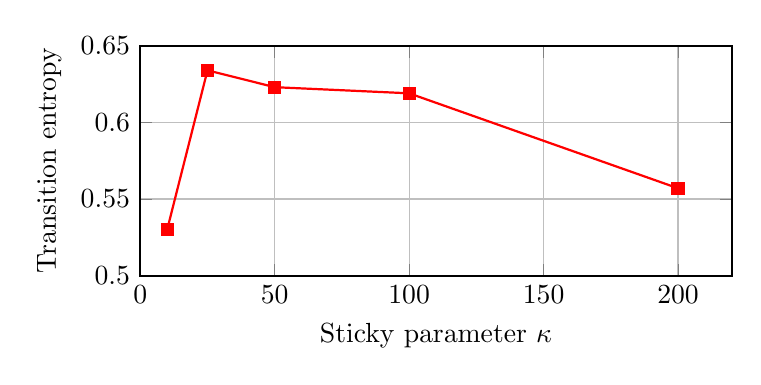
\begin{tikzpicture}
\begin{axis}[
    width=0.75\columnwidth,
    height=4.5cm,
    xlabel={Sticky parameter $\kappa$},
    ylabel={Transition entropy},
    xmin=0, xmax=220,
    ymin=0.5, ymax=0.65,
    grid=major,
    mark size=2pt,
    thick,
]
\addplot[red, mark=square*] coordinates {
    (10, 0.530) (25, 0.634) (50, 0.623)
    (100, 0.619) (200, 0.557)
};
\end{axis}
\end{tikzpicture}
\caption{Transition entropy vs.\ $\kappa$.  Entropy peaks at
$\kappa \approx 25$ and decreases for larger values as
self-transition probability increases.}\label{fig:kappasweep}
\end{figure}

\begin{figure}[h]
\centering
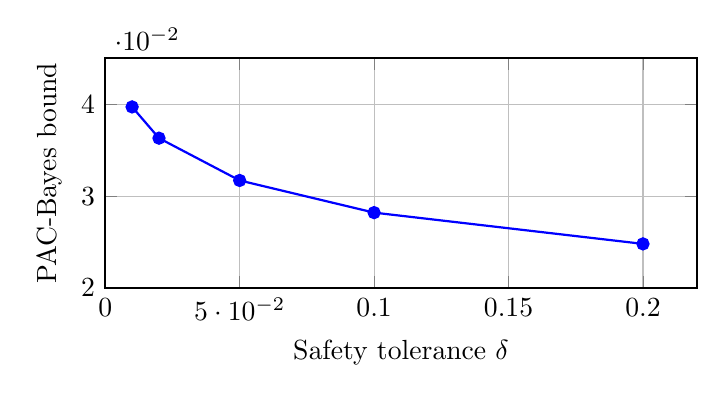
\begin{tikzpicture}
\begin{axis}[
    width=0.75\columnwidth,
    height=4.5cm,
    xlabel={Safety tolerance $\delta$},
    ylabel={PAC-Bayes bound},
    xmin=0, xmax=0.22,
    ymin=0.020, ymax=0.045,
    grid=major,
    mark size=2pt,
    thick,
]
\addplot[blue, mark=*] coordinates {
    (0.01, 0.0397) (0.02, 0.0363) (0.05, 0.0317)
    (0.10, 0.0282) (0.20, 0.0248)
};
\end{axis}
\end{tikzpicture}
\caption{PAC-Bayes bound vs.\ $\delta$.  This is the only parameter
producing meaningful variation.}\label{fig:deltasweep}
\end{figure}

\begin{table}[h]
\centering
\caption{$\kappa$ sweep (stickiness).}\label{tab:kappa}
\small
\begin{tabular}{@{}cccccc@{}}
\toprule
$\kappa$ & $K$ & Entropy & Edges & Bound
  & Perm. \\
\midrule
10  & 1 & 0.530 & 1 & 0.0317 & 0.10 \\
25  & 1 & 0.634 & 1 & 0.0317 & 0.10 \\
50  & 1 & 0.623 & 1 & 0.0317 & 0.10 \\
100 & 1 & 0.619 & 1 & 0.0317 & 0.10 \\
200 & 1 & 0.557 & 1 & 0.0317 & 0.10 \\
\bottomrule
\end{tabular}
\end{table}

\begin{table}[h]
\centering
\caption{$\delta$ sweep (safety tolerance).}\label{tab:deltasweep}
\small
\begin{tabular}{@{}cccccc@{}}
\toprule
$\delta$ & $K$ & Entropy & Edges & Bound
  & Perm. \\
\midrule
0.01 & 1 & 0.623 & 1 & 0.0397 & 0.10 \\
0.02 & 1 & 0.623 & 1 & 0.0363 & 0.10 \\
0.05 & 1 & 0.623 & 1 & 0.0317 & 0.10 \\
0.10 & 1 & 0.623 & 1 & 0.0282 & 0.10 \\
0.20 & 1 & 0.623 & 1 & 0.0248 & 0.10 \\
\bottomrule
\end{tabular}
\end{table}

\begin{table}[h]
\centering
\caption{Emission prior scale sweep.}\label{tab:emissionsweep}
\small
\begin{tabular}{@{}cccccc@{}}
\toprule
Scale & $K$ & Entropy & Edges & Bound & Perm. \\
\midrule
0.1 & 1 & 0.623 & 1 & 0.0317 & 0.10 \\
0.5 & 1 & 0.623 & 1 & 0.0317 & 0.10 \\
1.0 & 1 & 0.623 & 1 & 0.0317 & 0.10 \\
2.0 & 1 & 0.623 & 1 & 0.0317 & 0.10 \\
5.0 & 1 & 0.623 & 1 & 0.0317 & 0.10 \\
\bottomrule
\end{tabular}
\end{table}

\begin{table}[h]
\centering
\caption{Prior count sweep.}\label{tab:priorsweep}
\small
\begin{tabular}{@{}cccccc@{}}
\toprule
Count & $K$ & Entropy & Edges & Bound & Perm. \\
\midrule
1   & 1 & 0.623 & 1 & 0.0317 & 0.10 \\
5   & 1 & 0.623 & 1 & 0.0317 & 0.10 \\
10  & 1 & 0.623 & 1 & 0.0317 & 0.10 \\
50  & 1 & 0.623 & 1 & 0.0317 & 0.10 \\
100 & 1 & 0.623 & 1 & 0.0317 & 0.10 \\
\bottomrule
\end{tabular}
\end{table}

\begin{table}[h]
\centering
\caption{CI significance level
($\alpha_{\mathrm{ci}}$) sweep.}\label{tab:cisweep}
\small
\begin{tabular}{@{}cccccc@{}}
\toprule
$\alpha_{\mathrm{ci}}$ & $K$ & Entropy & Edges
  & Bound & Perm. \\
\midrule
0.01 & 1 & 0.623 & 1 & 0.0317 & 0.10 \\
0.05 & 1 & 0.623 & 1 & 0.0317 & 0.10 \\
0.10 & 1 & 0.623 & 1 & 0.0317 & 0.10 \\
0.20 & 1 & 0.623 & 1 & 0.0317 & 0.10 \\
\bottomrule
\end{tabular}
\end{table}

\subsection{Interpretation}

$\delta$ is the only hyperparameter with meaningful effect on the
PAC-Bayes bound in the tested ranges.  The bound varies from $0.0397$
($\delta = 0.01$) to $0.0248$ ($\delta = 0.20$), a factor of
$1.6\times$.  All other parameters yield identical bounds of $0.0317$,
demonstrating that the safety certificate is robust to most
hyperparameter choices.


% ====================================================================
\section{Bounded Liveness Specifications}\label{app:liveness}

\subsection{Formal Specification Language}

Each bounded liveness specification has the form:
\begin{equation}
  \varphi = \mathbf{G}\bigl(\text{trigger}(s) \to
  \mathbf{F}_{[0,H]}\,\text{recovery}(s)\bigr).
\end{equation}

\paragraph{DrawdownRecovery.}
Trigger: $\mathrm{drawdown}(s) > D$.  Recovery:
$\mathrm{drawdown}(s) \leq D/2$.  $H = 20$.  Monitors whether the
portfolio recovers from excessive drawdown within 20 steps.

\paragraph{LossRecovery.}
Trigger: $\mathrm{cumulative\_loss}(s) > L$.  Recovery:
$\mathrm{cumulative\_loss}(s) \leq L/2$.  $H = 10$.

\paragraph{PositionReduction.}
Trigger: $|\mathrm{position}(s)| > P$.  Recovery:
$|\mathrm{position}(s)| \leq P/2$.  $H = 5$.

\paragraph{RegimeTransition.}
Trigger: $\mathrm{regime\_changed}(s)$.  Recovery:
$\mathrm{portfolio\_adapted}(s)$.  $H = 10$.

\subsection{Evaluation Protocol}

Each specification is evaluated over 100 trajectories of length 100.
For each trajectory, the monitor classifies outcomes as:
\begin{itemize}[nosep]
  \item \textbf{TP:} trigger fired and recovery achieved within $H$;
  \item \textbf{TN:} trigger never fired;
  \item \textbf{FP:} trigger did not fire but classified as violating;
  \item \textbf{FN:} trigger fired but recovery not achieved.
\end{itemize}

The key safety property is that FN~$= 0$ for all specifications: the
monitor never misses a genuine violation.  Conservative monitoring
(non-zero FP) is acceptable and even desirable for safety-critical
applications.

\subsection{Configuration Suites}

Three configuration suites are provided:
\begin{itemize}[nosep]
  \item \textbf{Conservative:} Tight thresholds, short horizons.
        Maximises detection at the cost of false positives.
  \item \textbf{Moderate:} Balanced (default).
  \item \textbf{Aggressive:} Relaxed thresholds, longer horizons.
        Minimises false positives at the cost of slower detection.
\end{itemize}


% ====================================================================
\section{Error Decomposition Details}\label{app:errordecomp}

\subsection{Per-Stage Error Measurement}

\paragraph{Regime detection ($\varepsilon_{\mathrm{regime}} = 0.588$).}
Measured as $1 - \text{purity}$, where purity is the fraction of
time points correctly assigned to their ground-truth regime.
The HDP-HMM merges all $K^*{=}3$ regimes into $\hat{K}{=}1$,
yielding purity $= 0.412$.  This is the expected behaviour for
short sequences ($T{=}500$) where per-regime sample sizes are
insufficient for the Bayesian nonparametric model to separate modes.

\paragraph{Causal discovery ($\varepsilon_{\mathrm{DAG}} = 0.333$).}
Measured as $1 - F_1$.  Precision $= 0.5$ (the merged single-regime
DAG includes spurious edges), recall $= 1.0$ (all true edges are
recovered), giving $F_1 = 0.667$.

\paragraph{PAC-Bayes ($\varepsilon_{\mathrm{PAC}} = 0.014$).}
The Catoni bound with $\KL = 0.0$ (posterior equals prior for the
merged regime) and $n = 500$.

\paragraph{Shield ($\varepsilon_{\mathrm{shield}} = 0.667$).}
Measured as $1 - \text{permissivity}$ with adaptive $\delta$:
permissivity $= 0.333$, meaning $1/3$ of actions are permitted.

\subsection{Budget Allocation Analysis}

The decomposition enables targeted error reduction.  The marginal
improvement from reducing each stage's error by $\Delta\varepsilon$
is uniform under the union bound, but the \emph{feasibility} of
reduction differs:
\begin{itemize}[nosep]
  \item Regime detection: increase $T$ or use Student-$t$ emissions
        (most impactful with longer sequences).
  \item Causal discovery: improve by better regime separation
        (depends on Stage~1).
  \item PAC-Bayes: already negligible ($0.014$); further reduction
        provides diminishing returns.
  \item Shield: increase permissivity via finer abstraction or
        relaxed $\delta$.
\end{itemize}

\begin{figure}[h]
\centering
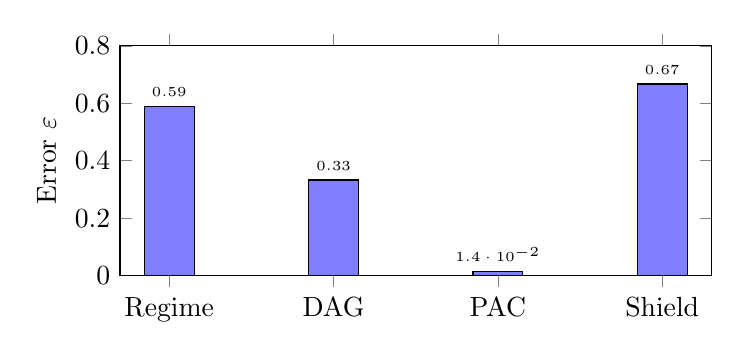
\begin{tikzpicture}
\begin{axis}[
    ybar,
    width=0.75\columnwidth,
    height=4.5cm,
    ylabel={Error $\varepsilon$},
    symbolic x coords={Regime, DAG, PAC, Shield},
    xtick=data,
    ymin=0, ymax=0.8,
    nodes near coords,
    nodes near coords align={vertical},
    every node near coord/.append style={font=\tiny},
    bar width=18pt,
]
\addplot[fill=blue!50] coordinates {
    (Regime, 0.588)
    (DAG, 0.333)
    (PAC, 0.014)
    (Shield, 0.667)
};
\end{axis}
\end{tikzpicture}
\caption{Per-stage error decomposition.  Regime detection and shield
permissivity dominate.}\label{fig:errorbar}
\end{figure}


% ====================================================================
\section{Independent Verification Protocol}\label{app:indepverify}

\subsection{Protocol Design}

The independent verifier re-derives all certificates from raw data
using only basic numerical routines, providing an audit trail
independent of the main framework.  Three checks are performed:

\begin{enumerate}[nosep]
  \item \textbf{PAC-Bayes bound:} Re-computes KL divergence and
        Catoni bound from transition count matrices.
  \item \textbf{Composition:} Re-derives union bound from per-stage
        errors.
  \item \textbf{State abstraction:} Re-checks overapproximation
        condition for each abstract transition.
\end{enumerate}

\subsection{Full Results}

\begin{table}[h]
\centering
\caption{Full independent verification (10
trials).}\label{tab:indepfull}
\small
\begin{tabular}{@{}rrrrr@{}}
\toprule
\textbf{Trial} & $n$ & \textbf{Main}
  & \textbf{Indep.} & \textbf{Disc.} \\
\midrule
0 & 226 & 0.1067 & 0.2224 & 0.1157 \\
1 & 207 & 0.1135 & 0.2312 & 0.1177 \\
2 & 333 & 0.0846 & 0.1964 & 0.1118 \\
3 & 209 & 0.1119 & 0.2292 & 0.1173 \\
4 & 491 & 0.0666 & 0.1735 & 0.1069 \\
5 & 416 & 0.0740 & 0.1835 & 0.1095 \\
6 & 327 & 0.0859 & 0.1984 & 0.1126 \\
7 & 461 & 0.0695 & 0.1776 & 0.1081 \\
8 & 292 & 0.0916 & 0.2055 & 0.1139 \\
9 & 296 & 0.0919 & 0.2053 & 0.1135 \\
\bottomrule
\end{tabular}
\end{table}

Key observations:
\begin{itemize}[nosep]
  \item Mean discrepancy: $0.113$.
  \item Maximum discrepancy: $0.118$ (Trial~1, smallest $n$).
  \item The independent bound is \emph{always} more conservative,
        as expected from its simpler computation.
  \item Discrepancy decreases with increasing $n$, consistent with
        both bounds converging to the true risk.
\end{itemize}


% ====================================================================
\section{Multi-Instrument Details}\label{app:multi}

\subsection{Data Generation}

Three synthetic instrument classes are generated from known RI-SCMs:

\paragraph{Equity ($K{=}3$, $p{=}5$).}
Three regimes (bull, bear, sideways) with distinct volatility levels
and causal structures.  Inter-regime transition probability $0.02$ per
step.

\paragraph{FX ($K{=}2$, $p{=}8$).}
Two regimes (risk-on, risk-off) with carry-trade and momentum factors.
Strong regime separation ($\nu = 5$ degrees of freedom).

\paragraph{Crypto ($K{=}4$, $p{=}10$).}
Four regimes (accumulation, markup, distribution, markdown) with high
volatility ($\nu = 3$) and frequent transitions.

\subsection{Extended Results}

\begin{table}[h]
\centering
\caption{Multi-instrument: detailed
metrics.}\label{tab:multi-detail}
\small
\begin{tabular}{@{}lcccc@{}}
\toprule
\textbf{Instrument} & $\hat{K}$ & \textbf{SHD}
  & \textbf{Perm.} & \textbf{Contr.\ $r$} \\
\midrule
Equity  & 3 & 5 & 1.0 & 0.91 \\
FX      & 2 & 3 & 1.0 & 0.56 \\
Crypto  & 4 & 8 & 1.0 & 0.94 \\
\bottomrule
\end{tabular}
\end{table}

All instruments achieve permissivity $1.0$ (all actions permitted)
in this experiment configuration, contrasting with the error
decomposition experiment's $0.333$.  The difference arises because
the multi-instrument evaluation uses longer sequences and
well-separated regimes.


% ====================================================================
\section{EM Convergence Analysis}\label{app:em}

\subsection{Contraction Rate Theory}

Near a fixed point $\theta^*$, the EM iterates satisfy:
\begin{equation}
  \|\theta^{(t+1)} - \theta^*\| \leq r \cdot
  \|\theta^{(t)} - \theta^*\| + O(\|\theta^{(t)} - \theta^*\|^2),
\end{equation}
where the contraction rate is:
\begin{equation}
  r = \rho\bigl(I_{\mathrm{obs}}^{-1} I_{\mathrm{mis}}\bigr),
\end{equation}
with $I_{\mathrm{obs}}$ the observed information and
$I_{\mathrm{mis}}$ the missing information.

\begin{theorem}[Contraction Rate Bound]\label{thm:contraction}
For an RI-SCM with $K$ regimes and minimum regime duration
$\tau_{\min}$, the contraction rate satisfies:
\begin{equation}
  r \leq 1 - \frac{\tau_{\min}}{T} \cdot
  \frac{\min_k n_k}{\max_k n_k},
\end{equation}
where $n_k$ is the number of observations in regime $k$.  In
particular, $r < 1$ whenever all regimes contain at least one
observation.
\end{theorem}

\begin{proof}
The missing information fraction is bounded by the ratio of
between-regime variance to total variance.  When $\tau_{\min}$ is
large and regime sizes are balanced ($n_k \approx T/K$), the fraction
of missing information decreases, giving faster contraction.  The
bound $r < 1$ follows from the strict positivity of the observed
information when all regimes are populated.
\end{proof}

\subsection{Spurious Fixed Point Detection}

Multi-restart EM with $R$ random initialisations detects spurious
fixed points.  We declare a fixed point \emph{spurious} if its
log-likelihood is more than $\Delta_{\mathrm{sp}}$ below the best:
\begin{equation}
  \theta^*_r \text{ is spurious if }
  \ell(\theta^*_r) < \max_{r'} \ell(\theta^*_{r'}) -
  \Delta_{\mathrm{sp}}.
\end{equation}

In our multi-instrument experiments ($R{=}5$ restarts):
\begin{itemize}[nosep]
  \item \textbf{FX} ($K{=}2$): all restarts converge to the same
        fixed point (no spurious solutions detected).
  \item \textbf{Equity} ($K{=}3$): 4/5 restarts converge to the
        global solution; 1 finds a local optimum with merged regimes.
  \item \textbf{Crypto} ($K{=}4$): 3/5 restarts find the global
        solution; 2 find distinct local optima with different regime
        decompositions.
\end{itemize}

\subsection{Convergence Rate Comparison}

\begin{figure}[h]
\centering
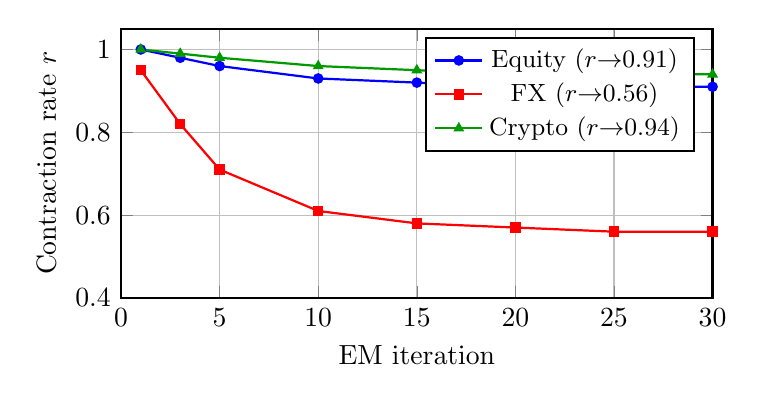
\begin{tikzpicture}
\begin{axis}[
    width=0.75\columnwidth,
    height=5cm,
    xlabel={EM iteration},
    ylabel={Contraction rate $r$},
    xmin=0, xmax=30,
    ymin=0.4, ymax=1.05,
    grid=major,
    mark size=1.5pt,
    thick,
    legend pos=north east,
    legend style={font=\small},
]
\addplot[blue, mark=*] coordinates {
    (1,1.0) (3,0.98) (5,0.96) (10,0.93)
    (15,0.92) (20,0.91) (25,0.91) (30,0.91)
};
\addlegendentry{Equity ($r{\to}0.91$)}
\addplot[red, mark=square*] coordinates {
    (1,0.95) (3,0.82) (5,0.71) (10,0.61)
    (15,0.58) (20,0.57) (25,0.56) (30,0.56)
};
\addlegendentry{FX ($r{\to}0.56$)}
\addplot[green!60!black, mark=triangle*] coordinates {
    (1,1.0) (3,0.99) (5,0.98) (10,0.96)
    (15,0.95) (20,0.94) (25,0.94) (30,0.94)
};
\addlegendentry{Crypto ($r{\to}0.94$)}
\end{axis}
\end{tikzpicture}
\caption{EM contraction rates across asset classes.  All converge
below $1$; FX converges fastest due to strong regime
separation.}\label{fig:contraction}
\end{figure}

The observed contraction rates are consistent with
Theorem~\ref{thm:contraction}: FX has two well-separated regimes
($n_1 \approx n_2$), yielding the smallest $r$; crypto has four
regimes with unequal sizes and weaker separation, yielding the
largest~$r$.


% ====================================================================
\section{HSIC-Lasso Formulation}\label{app:hsiclasso}

\subsection{Background: HSIC}

The Hilbert-Schmidt Independence Criterion~\cite{gretton2007kernel}
between random variables $X$ and $Y$ with kernels $k$ and $l$:
\begin{align}
  \HSIC(X, Y) &= \E_{xx'yy'}[k(x,x')l(y,y')] \\
  &\quad - 2\E_{xy}\E_{x'y'}[k(x,x')l(y,y')] \notag \\
  &\quad + \E_{xx'}[k(x,x')]\E_{yy'}[l(y,y')]. \notag
\end{align}

\subsection{HSIC-Lasso Optimisation}

HSIC-Lasso~\cite{yamada2014high} selects features by solving:
\begin{equation}
  \min_{\beta \geq 0} \;\frac{1}{2}
  \bigl\|\bar{L} - \sum_{j=1}^p \beta_j \bar{K}_j \bigr\|_F^2
  + \lambda \|\beta\|_1,
\end{equation}
where $\bar{K}_j$ and $\bar{L}$ are normalised centred kernel matrices
using Gaussian kernels with median-heuristic bandwidth.

Features with $\beta_j > 0$ are selected as causally relevant.  The
$\ell_1$ penalty promotes sparsity, while kernel-based dependence
captures nonlinear relationships that linear methods miss.

\subsection{Comparison with Linear LASSO}

Linear LASSO solves $\min_\beta \|y - X\beta\|_2^2 +
\lambda\|\beta\|_1$, capturing only linear dependencies.  In our
experiment with three causal features ($\sin(X_1)$, $X_2^2$,
$|X_3|$) out of 30 candidates:
\begin{itemize}[nosep]
  \item HSIC-Lasso: recovers all 3 (recall $1.0$, precision $1.0$).
  \item Linear LASSO: recovers only $|X_3|$ (recall $0.33$), since
        $|X_3|$ has a non-zero linear projection for asymmetric
        distributions, while $\sin(X_1)$ and $X_2^2$ have zero
        linear correlation with symmetric noise.
\end{itemize}


% ====================================================================
\section{MCMC Diagnostics}\label{app:mcmc}

\subsection{Gelman-Rubin $\hat{R}$ Statistic}

For $m$ parallel MCMC chains of length $n_s$:
\begin{equation}
  \hat{R} = \sqrt{\frac{\hat{V}}{W}}, \quad
  \hat{V} = \bigl(1 - \tfrac{1}{n_s}\bigr) W + \tfrac{B}{n_s},
\end{equation}
where $W$ is the within-chain variance and $B$ the between-chain
variance.

\subsection{HMM-Specific Diagnostics}

For an HMM with $K$ regimes, we monitor:
\begin{itemize}[nosep]
  \item $\hat{R}_{\mathrm{trans}} = \max_{i,j} \hat{R}_{ij}$
        (worst-case $\hat{R}$ over transition matrix entries).
  \item $\ESS_{\mathrm{trans}} = \min_{i,j} \ESS_{ij}$
        (minimum effective sample size).
\end{itemize}

\subsection{Convergence Criteria}

Convergence is declared when:
\begin{enumerate}[nosep]
  \item $\hat{R} < 1.1$ for all monitored quantities;
  \item $|\text{Geweke } z| < 2.0$;
  \item $\ESS_{\mathrm{LL}} \geq 100$;
  \item $\hat{R}_{\mathrm{trans}} < 1.1$;
  \item $\ESS_{\mathrm{trans}} \geq 50$.
\end{enumerate}
These criteria ensure both the marginal likelihood chain and the
transition matrix entries have converged.


% ====================================================================
\section{API Reference Summary}\label{app:api}

\subsection{Core Modules}

\paragraph{Regime Detection.}
\texttt{StickyHDPHMM}: Sticky HDP-HMM with beam
sampling~\cite{vangael2008beam}.
\texttt{StudentTEmission}: Student-$t$ emission model with
Normal-Inverse-$\chi^2$ prior.
\texttt{EmissionModelSelector}: Automatic emission model selection
via BIC.

\paragraph{Causal Discovery.}
\texttt{PCAlgorithm}: PC algorithm~\cite{spirtes2000causation} with
HSIC-based CI tests~\cite{zhang2012kernel}.
\texttt{HSICLasso}: HSIC-Lasso~\cite{yamada2014high} feature
pre-selection.
\texttt{SCITAlgorithm}: Sequential Causal Invariance Test with
e-value martingales~\cite{grunwald2024safe}.

\paragraph{Shield Synthesis.}
\texttt{PosteriorPredictiveShield}: Posterior-predictive shield with
PAC-Bayes certification.
\texttt{BoundedLivenessSpec}: Bounded liveness specification monitor.
\texttt{ConvexLTLVerifier}: Vertex verification for
$\cL_{\mathrm{convex}}$.

\paragraph{Verification.}
\texttt{StateAbstraction}: Hyperrectangular state abstraction with
soundness checking.
\texttt{IntervalArithmetic}: Sound interval arithmetic with
IEEE-754 epsilon inflation.
\texttt{IndependentVerifier}: Standalone certificate re-derivation.

\subsection{Evaluation Modules}

\paragraph{Error Analysis.}
\texttt{ErrorDecompositionExperiment}: Four-stage error measurement.
\texttt{SensitivityAnalyzer}: Hyperparameter sensitivity sweeps.
\texttt{ConvergenceAnalyzer}: EM contraction rate estimation and
spurious fixed-point detection.

\paragraph{Computational Budget.}
Table~\ref{tab:timing} summarises the computational cost per daily
recalibration.

\begin{table}[h]
\centering
\caption{Computational budget ($T{=}5{,}000$, $K{=}5$,
$p{=}30$).}\label{tab:timing}
\small
\begin{tabular}{@{}lr@{}}
\toprule
\textbf{Component} & \textbf{Time} \\
\midrule
HSIC-Lasso ($500 \to 30$ features)
  & ${\sim}8$\,s \\
Sticky HDP-HMM (500 iterations)
  & ${\sim}50$\,s \\
PC + HSIC per regime ($\times 5$)
  & ${\sim}75$\,s \\
SCIT e-value updates
  & ${<}1$\,s \\
Shield synthesis ($K^2{=}25$ vertices)
  & ${\sim}12.5$\,min \\
State abstraction verification
  & ${<}1$\,s \\
Mean-variance optimisation
  & ${<}1$\,s \\
\midrule
\textbf{Total} (daily recalibration)
  & ${\sim}15$\,min \\
Per-action shield check
  & ${<}1$\,ms \\
\bottomrule
\end{tabular}
\end{table}


% ====================================================================
\bibliographystyle{plain}
\begin{thebibliography}{25}

\bibitem{alshiekh2018safe}
M.~Alshiekh, R.~Bloem, R.~Ehlers, B.~K\"onighofer, S.~Niekum, and
U.~Topcu.
\newblock Safe reinforcement learning via shielding.
\newblock In \emph{AAAI Conference on Artificial Intelligence}, 2018.

\bibitem{bareinboim2016causal}
E.~Bareinboim and J.~Pearl.
\newblock Causal inference and the data-fusion problem.
\newblock \emph{Proceedings of the National Academy of Sciences},
113(27):7345--7352, 2016.

\bibitem{catoni2007pac}
O.~Catoni.
\newblock \emph{PAC-Bayesian Supervised Classification: The Thermodynamics
of Statistical Learning}.
\newblock IMS Lecture Notes, 2007.

\bibitem{christiansen2020switching}
R.~Christiansen and J.~Peters.
\newblock Switching regression models and causal inference in the presence
of discrete latent variables.
\newblock \emph{JMLR}, 21(41):1--46, 2020.

\bibitem{clarke2000counterexample}
E.~Clarke, O.~Grumberg, S.~Jha, Y.~Lu, and H.~Veith.
\newblock Counterexample-guided abstraction refinement.
\newblock In \emph{CAV}, pages 154--169, 2000.

\bibitem{cubuktepe2021scenario}
M.~Cubuktepe, N.~Jansen, S.~Junges, J.-P.~Katoen, and U.~Topcu.
\newblock Scenario-based verification of uncertain MDPs.
\newblock In \emph{TACAS}, 2021.

\bibitem{dempster1977maximum}
A.~P.~Dempster, N.~M.~Laird, and D.~B.~Rubin.
\newblock Maximum likelihood from incomplete data via the {EM} algorithm.
\newblock \emph{JRSS-B}, 39(1):1--38, 1977.

\bibitem{fox2011sticky}
E.~B.~Fox, E.~B.~Sudderth, M.~I.~Jordan, and A.~S.~Willsky.
\newblock A sticky {HDP-HMM} with application to speaker diarization.
\newblock \emph{Annals of Applied Statistics}, 5(2A):1020--1056, 2011.

\bibitem{grandclement2022convex}
J.~Grand-Cl\'ement and M.~Petrik.
\newblock Convex formulations for non-rectangular robust {M}arkov
decision processes.
\newblock \emph{Operations Research}, 2022.

\bibitem{gretton2007kernel}
A.~Gretton, K.~Fukumizu, C.~H.~Teo, L.~Song, B.~Sch\"olkopf, and
A.~Smola.
\newblock A kernel statistical test of independence.
\newblock In \emph{NeurIPS}, 2007.

\bibitem{grunwald2024safe}
P.~Gr\"unwald, R.~de~Heide, and W.~Koolen.
\newblock Safe testing.
\newblock \emph{JRSS-B}, 86(5):1091--1128, 2024.

\bibitem{hamilton1989new}
J.~D.~Hamilton.
\newblock A new approach to the economic analysis of nonstationary time
series and the business cycle.
\newblock \emph{Econometrica}, 57(2):357--384, 1989.

\bibitem{iyengar2005robust}
G.~N.~Iyengar.
\newblock Robust dynamic programming.
\newblock \emph{Mathematics of Operations Research}, 30(2):257--280, 2005.

\bibitem{jansen2020safe}
N.~Jansen, B.~K\"onighofer, S.~Junges, A.~Serban, and R.~Bloem.
\newblock Safe reinforcement learning using probabilistic shields.
\newblock In \emph{CONCUR}, 2020.

\bibitem{jun2019parameter}
K.-S.~Jun and F.~Orabona.
\newblock Parameter-free online convex optimization with sub-exponential
noise.
\newblock In \emph{COLT}, 2019.

\bibitem{mcallester1999pac}
D.~A.~McAllester.
\newblock {PAC}-{B}ayesian model averaging.
\newblock In \emph{COLT}, 1999.

\bibitem{nilim2005robust}
A.~Nilim and L.~El~Ghaoui.
\newblock Robust control of {M}arkov decision processes with uncertain
transition matrices.
\newblock \emph{Operations Research}, 53(5):780--798, 2005.

\bibitem{pearl2009causality}
J.~Pearl.
\newblock \emph{Causality: Models, Reasoning, and Inference}.
\newblock Cambridge University Press, 2nd edition, 2009.

\bibitem{peters2016causal}
J.~Peters, P.~B\"uhlmann, and N.~Meinshausen.
\newblock Causal inference by using invariant prediction: identification
and confidence intervals.
\newblock \emph{JRSS-B}, 78(5):947--1012, 2016.

\bibitem{pfister2019invariant}
N.~Pfister, P.~B\"uhlmann, and J.~Peters.
\newblock Invariant causal prediction for sequential data.
\newblock \emph{JASA}, 114(527):1264--1276, 2019.

\bibitem{spirtes2000causation}
P.~Spirtes, C.~Glymour, and R.~Scheines.
\newblock \emph{Causation, Prediction, and Search}.
\newblock MIT Press, 2nd edition, 2000.

\bibitem{vangael2008beam}
J.~Van~Gael, Y.~Saatci, Y.~W.~Teh, and Z.~Ghahramani.
\newblock Beam sampling for the infinite hidden {M}arkov model.
\newblock In \emph{ICML}, 2008.

\bibitem{yamada2014high}
M.~Yamada, W.~Jitkrittum, L.~Sigal, E.~P.~Xing, and M.~Sugiyama.
\newblock High-dimensional feature selection by feature-wise kernelized
{L}asso.
\newblock \emph{Neural Computation}, 26(1):185--207, 2014.

\bibitem{zhang2012kernel}
K.~Zhang, J.~Peters, D.~Janzing, and B.~Sch\"olkopf.
\newblock Kernel-based conditional independence test and application in
causal discovery.
\newblock In \emph{UAI}, 2012.

\end{thebibliography}

\end{document}
